%% ============================================================
%% DVB-S2 ACM — Simulation & Hardware Results
%% NUS Beamer Theme | Author: Pasindu Manujaya
%% ============================================================
\documentclass[aspectratio=169,10pt]{beamer}
\usepackage[utf8]{inputenc}
\usepackage[T1]{fontenc}
\usepackage{amsmath,amssymb}
\usepackage{graphicx}
\graphicspath{{figures/}}
\usepackage{booktabs}
\usepackage{array}
\usepackage{xcolor}
\usepackage{tikz}
\usetikzlibrary{shapes.geometric,arrows.meta,positioning,fit,backgrounds,calc}
\usepackage{hyperref}
\usepackage{multimedia}
\usepackage{colortbl}
\usepackage{multirow}
\usepackage[most]{tcolorbox}

% ── NUS Colours ─────────────────────────────────────────────
\definecolor{NUSblue}{HTML}{003D7C}
\definecolor{NUSorange}{HTML}{EF7C00}
\definecolor{NUSlightblue}{HTML}{006CB7}
\definecolor{NUSgray}{HTML}{58595B}
\definecolor{NUSlightgray}{HTML}{F4F4F4}
\definecolor{NUSgreen}{HTML}{009F6B}
\definecolor{NUSred}{HTML}{C0392B}

% ── tcolorbox environments ───────────────────────────────────
\newtcolorbox{keybox}[1]{
  colback=NUSorange!10, colframe=NUSorange!80,
  title={\textbf{#1}}, fonttitle=\bfseries\small,
  arc=4pt, left=6pt, right=6pt, top=4pt, bottom=4pt,
}
\newtcolorbox{resultbox}[1]{
  colback=NUSgreen!8, colframe=NUSgreen!70,
  title={\textbf{#1}}, fonttitle=\bfseries\small,
  arc=4pt, left=6pt, right=6pt, top=4pt, bottom=4pt,
}
\newtcolorbox{notebox}[1]{
  colback=NUSlightgray, colframe=NUSgray!60,
  title={\textbf{#1}}, fonttitle=\bfseries\small,
  arc=4pt, left=6pt, right=6pt, top=4pt, bottom=4pt,
}

% ── Beamer Theme ─────────────────────────────────────────────
\usetheme{Madrid}
\usecolortheme[named=NUSblue]{structure}
\setbeamercolor{palette primary}{bg=NUSblue,fg=white}
\setbeamercolor{palette secondary}{bg=NUSlightblue,fg=white}
\setbeamercolor{palette tertiary}{bg=NUSblue!80,fg=white}
\setbeamercolor{palette quaternary}{bg=NUSblue,fg=white}
\setbeamercolor{frametitle}{bg=NUSblue,fg=white}
\setbeamercolor{title}{fg=white}
\setbeamercolor{block title}{bg=NUSorange,fg=white}
\setbeamercolor{block body}{bg=NUSorange!10}
\setbeamerfont{frametitle}{series=\bfseries,size=\normalsize}
\setbeamerfont{title}{series=\bfseries,size=\Large}
\setbeamertemplate{navigation symbols}{}
\setbeamertemplate{footline}{
  \leavevmode\hbox{%
    \begin{beamercolorbox}[wd=.33\paperwidth,ht=2.5ex,dp=1ex,center]{palette primary}
      \usebeamerfont{author in head/foot}\insertshortauthor
    \end{beamercolorbox}%
    \begin{beamercolorbox}[wd=.34\paperwidth,ht=2.5ex,dp=1ex,center]{palette secondary}
      \usebeamerfont{title in head/foot}\insertshorttitle
    \end{beamercolorbox}%
    \begin{beamercolorbox}[wd=.33\paperwidth,ht=2.5ex,dp=1ex,center]{palette primary}
      \usebeamerfont{date in head/foot}
      \insertframenumber\,/\,\inserttotalframenumber
    \end{beamercolorbox}}%
}

% ── Title Info ───────────────────────────────────────────────
\title[DVB-S2 ACM Results]{DVB-S2 ACM with AI/ML Cognitive Engine\\[0.3em]
\normalsize Simulation \& GNU Radio Hardware Results}
\author[Pasindu Manujaya]{Pasindu Manujaya}
\institute[NUS]{National University of Singapore}
\date{March 2026}

%% ============================================================
\begin{document}
%% ============================================================

% ── Title Slide ──────────────────────────────────────────────
\begin{frame}
\titlepage
\vspace{-0.5em}
\begin{center}
\small
\textcolor{NUSgray}{LEO X-Band Link $\cdot$ 500 km $\cdot$ 8.025 GHz $\cdot$ USRP B200 + GNU Radio 3.10}
\end{center}
\end{frame}

% ── High-Level System Architecture ─── MOVED TO SLIDE 2 ──────
\begin{frame}{High-Level System Architecture}
  \begin{center}
  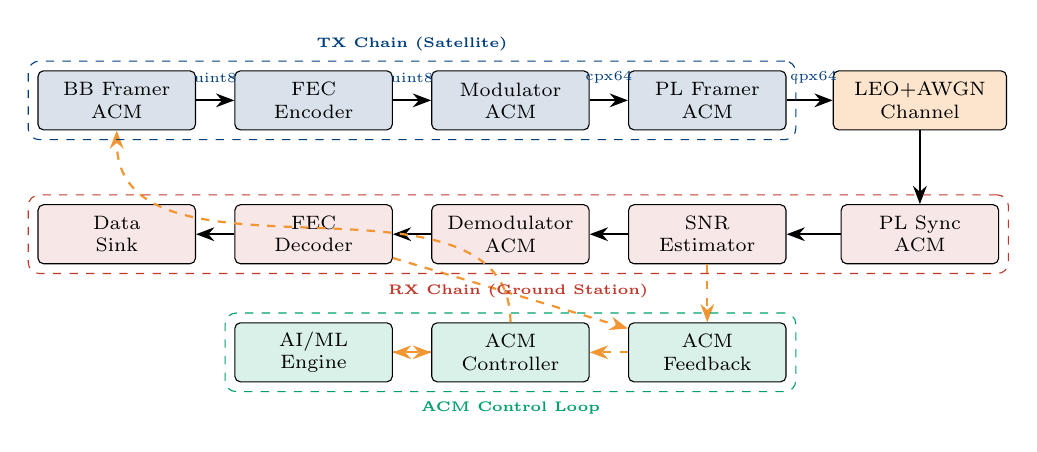
\begin{tikzpicture}[
    block/.style={rectangle,draw,fill=NUSblue!15,minimum width=2.0cm,
                  minimum height=0.75cm,align=center,font=\scriptsize,rounded corners=2pt},
    rblock/.style={rectangle,draw,fill=NUSred!12,minimum width=2.0cm,
                   minimum height=0.75cm,align=center,font=\scriptsize,rounded corners=2pt},
    cblock/.style={rectangle,draw,fill=NUSgreen!15,minimum width=2.0cm,
                   minimum height=0.75cm,align=center,font=\scriptsize,rounded corners=2pt},
    chblock/.style={rectangle,draw,fill=NUSorange!20,minimum width=2.2cm,
                    minimum height=0.75cm,align=center,font=\scriptsize,rounded corners=2pt},
    arr/.style={-Stealth,thick},
    msgarr/.style={-Stealth,thick,dashed,NUSorange!80},
  ]
  \node[block]  (bbf)  at (0,3.5)   {BB Framer\\ACM};
  \node[block]  (fece) at (2.5,3.5) {FEC\\Encoder};
  \node[block]  (mod)  at (5.0,3.5) {Modulator\\ACM};
  \node[block]  (plf)  at (7.5,3.5) {PL Framer\\ACM};
  \node[chblock](ch)   at (10.2,3.5){LEO+AWGN\\Channel};
  \node[rblock] (pls)  at (10.2,1.8){PL Sync\\ACM};
  \node[rblock] (snr)  at (7.5,1.8) {SNR\\Estimator};
  \node[rblock] (dem)  at (5.0,1.8) {Demodulator\\ACM};
  \node[rblock] (fecd) at (2.5,1.8) {FEC\\Decoder};
  \node[rblock] (sink) at (0,1.8)   {Data\\Sink};
  \node[cblock] (acmfb)at (7.5,0.3) {ACM\\Feedback};
  \node[cblock] (acmc) at (5.0,0.3) {ACM\\Controller};
  \node[cblock] (ai)   at (2.5,0.3) {AI/ML\\Engine};
  \draw[arr] (bbf)--(fece); \draw[arr] (fece)--(mod);
  \draw[arr] (mod)--(plf);  \draw[arr] (plf)--(ch);
  \draw[arr] (ch)--(pls);
  \draw[arr] (pls)--(snr);  \draw[arr] (snr)--(dem);
  \draw[arr] (dem)--(fecd); \draw[arr] (fecd)--(sink);
  \draw[msgarr] (snr)--(acmfb); \draw[msgarr] (fecd)--(acmfb);
  \draw[msgarr] (acmfb)--(acmc); \draw[msgarr] (acmc)--(ai);
  \draw[msgarr] (ai)--(acmc);
  \draw[msgarr] (acmc.north) to[out=90,in=270] (bbf.south);
  \node[font=\tiny,NUSblue,above] at (1.25,3.6) {uint8};
  \node[font=\tiny,NUSblue,above] at (3.75,3.6) {uint8};
  \node[font=\tiny,NUSblue,above] at (6.25,3.6) {cpx64};
  \node[font=\tiny,NUSblue,above] at (8.85,3.6) {cpx64};
  \node[draw=NUSblue,dashed,rounded corners,fit=(bbf)(plf),
        label={[font=\tiny\bfseries,NUSblue]above:TX Chain (Satellite)}] {};
  \node[draw=NUSred,dashed,rounded corners,fit=(pls)(sink),
        label={[font=\tiny\bfseries,NUSred]below:RX Chain (Ground Station)}] {};
  \node[draw=NUSgreen,dashed,rounded corners,fit=(acmfb)(ai),
        label={[font=\tiny\bfseries,NUSgreen]below:ACM Control Loop}] {};
  \end{tikzpicture}
  \end{center}
  \vspace{-0.2em}
  \begin{columns}
    \begin{column}{0.5\textwidth}
      \scriptsize \textbf{Stream tag path (in-band, zero latency):}\\
      BB Framer attaches \texttt{"modcod"} tag to frame start $\Rightarrow$\\
      every downstream block reads tag and applies correct constellation/FEC.
    \end{column}
    \begin{column}{0.46\textwidth}
      \scriptsize \textbf{Message port path (out-of-band, ACM feedback):}\\
      SNR + BER/FER $\Rightarrow$ ACM Feedback $\Rightarrow$ Controller $\Rightarrow$\\
      DQN/rule-based $\Rightarrow$ new MODCOD $\Rightarrow$ BB Framer.
    \end{column}
  \end{columns}
\end{frame}

% ── Two-Tool Strategy ─── MOVED TO SLIDE 3 ───────────────────
\begin{frame}[shrink=5]{Two-Tool Validation Strategy}
\begin{columns}[T]
  \begin{column}{0.48\textwidth}
    \begin{block}{\texttt{acm\_loopback\_sim.py} — Algorithm validation}
      \begin{itemize}\small
        \item Pure Python — no compilation needed
        \item \textbf{Runs in seconds} — full LEO pass in $\sim$2 s
        \item Same 52-dim DQN + PER as production AI engine
        \item BER/FER from waterfall lookup table (approximation)
        \item SNR: true value + 0.3\,dB Gaussian noise model
        \item Zero ACM loop latency
      \end{itemize}
    \end{block}
    \vspace{0.4em}
    \begin{notebox}{Use when}
      \small Tuning hyperparameters, comparing strategies, generating paper plots — anywhere speed matters more than signal accuracy.
    \end{notebox}
  \end{column}
  \begin{column}{0.48\textwidth}
    \begin{alertblock}{\texttt{acm\_loopback.grc} — System validation}
      \begin{itemize}\small
        \item Random source $\to$ full IQ chain (BCH+LDPC, modulation, PL sync)
        \item \textbf{Real LDPC decoding} — actual bit errors counted
        \item Real Pilot-MMSE + M2M4 + Kalman SNR estimation
        \item PLSCODE signalling per PL frame
        \item ACM feedback latency: $\sim$100\,ms report period
        \item Currently software loopback — USRP B200 next
      \end{itemize}
    \end{alertblock}
    \vspace{0.4em}
    \begin{resultbox}{Use when}
      \small Validating the signal chain, demonstrating the live system, preparing for USRP B200 hardware (IoV March 2026).
    \end{resultbox}
  \end{column}
\end{columns}
\vspace{0.4em}
\begin{center}
\small\textcolor{NUSgray}{Both tools use the \textbf{same DQNAgent} from \texttt{acm\_controller\_ai.py} — results are consistent by design.}
\end{center}
\end{frame}

% ── DQN Architecture ─── MOVED TO SLIDE 4 ────────────────────
\begin{frame}[shrink=5,fragile]{AI/ML Engine: Dueling Double DQN}
\begin{columns}[T]
  \begin{column}{0.38\textwidth}
    \begin{alertblock}{Why Reinforcement Learning?}
      \small
      ACM is a \textbf{sequential decision problem} — the controller must
      choose a MODCOD at every frame based on channel history, and the
      consequence (BER, FER) only appears one step later.\\[0.4em]
      \textbf{Reinforcement Learning (RL)} is the natural framework:
      the agent learns by trial-and-error, receiving a reward signal
      after each action, without needing a labelled dataset.\\[0.4em]
      \textbf{DQN (Deep Q-Network)} is the specific RL algorithm used
      in this research — it approximates the optimal action-value
      function $Q^*(s,a)$ using a deep neural network.
    \end{alertblock}
  \end{column}
  \begin{column}{0.60\textwidth}
    \begin{center}
    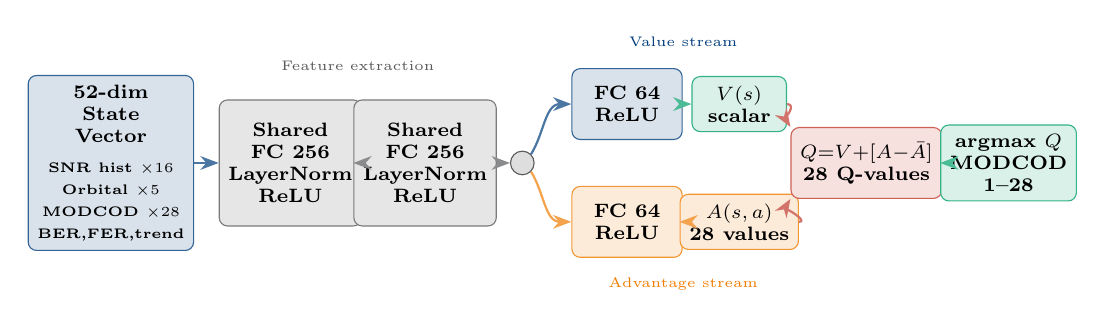
\begin{tikzpicture}[xscale=0.95, yscale=0.88,
        box/.style={rectangle, draw=#1!80, fill=#1!15, rounded corners=3pt,
                    minimum width=1.6cm, minimum height=0.55cm,
                    align=center, font=\scriptsize\bfseries},
        arr/.style={-Stealth, thick, #1!70},
      ]
      \node[box=NUSblue, minimum width=2.0cm, minimum height=2.2cm,
            align=center, font=\scriptsize\bfseries] (inp) at (0,0)
        {52-dim\\State\\Vector\\[0.3em]
         \tiny SNR hist $\times16$\\
         \tiny Orbital $\times5$\\
         \tiny MODCOD $\times28$\\
         \tiny BER,FER,trend};
      \node[box=NUSgray, minimum width=1.5cm, minimum height=1.6cm] (h1) at (2.4,0)
        {Shared\\FC 256\\LayerNorm\\ReLU};
      \node[box=NUSgray, minimum width=1.5cm, minimum height=1.6cm] (h2) at (4.2,0)
        {Shared\\FC 256\\LayerNorm\\ReLU};
      \node[circle, draw=NUSgray, fill=NUSgray!20,
            minimum size=0.3cm, inner sep=1pt] (fork) at (5.5,0) {};
      \node[box=NUSblue, minimum width=1.4cm, minimum height=0.9cm] (vfc) at (6.9, 0.85)
        {FC 64\\ReLU};
      \node[box=NUSgreen, minimum width=1.2cm, minimum height=0.55cm] (vs) at (8.4, 0.85)
        {$V(s)$\\scalar};
      \node[box=NUSorange, minimum width=1.4cm, minimum height=0.9cm] (afc) at (6.9,-0.85)
        {FC 64\\ReLU};
      \node[box=NUSorange, minimum width=1.2cm, minimum height=0.7cm] (as) at (8.4,-0.85)
        {$A(s,a)$\\28 values};
      \node[box=NUSred, minimum width=1.6cm, minimum height=0.9cm] (q) at (10.1, 0)
        {$Q{=}V{+}[A{-}\bar{A}]$\\28 Q-values};
      \node[box=NUSgreen, minimum width=1.5cm, minimum height=0.7cm] (out) at (12.0,0)
        {argmax $Q$\\MODCOD\\1--28};
      \draw[arr=NUSblue]  (inp.east) -- (h1.west);
      \draw[arr=NUSgray]  (h1.east)  -- (h2.west);
      \draw[arr=NUSgray]  (h2.east)  -- (fork.west);
      \draw[arr=NUSblue]  (fork.north east) to[out=60,in=180]  (vfc.west);
      \draw[arr=NUSorange](fork.south east) to[out=-60,in=180] (afc.west);
      \draw[arr=NUSgreen] (vfc.east)  -- (vs.west);
      \draw[arr=NUSorange](afc.east)  -- (as.west);
      \draw[arr=NUSred]   (vs.east)   to[out=0,in=120]  (q.north west);
      \draw[arr=NUSred]   (as.east)   to[out=0,in=-120] (q.south west);
      \draw[arr=NUSgreen] (q.east)    -- (out.west);
      \node[font=\tiny, NUSgray]   at (3.3, 1.4)  {Feature extraction};
      \node[font=\tiny, NUSblue]   at (7.65, 1.75) {Value stream};
      \node[font=\tiny, NUSorange] at (7.65,-1.75) {Advantage stream};
    \end{tikzpicture}
    \end{center}
    \vspace{0.3em}
    \begin{columns}[T]
      \begin{column}{0.48\textwidth}
        \begin{keybox}{Dueling heads}
          \scriptsize Separates \textit{how good is this state} ($V$) from
          \textit{how much better is this action} ($A$). More stable learning
          than a single Q head.
        \end{keybox}
      \end{column}
      \begin{column}{0.48\textwidth}
        \begin{resultbox}{Double DQN}
          \scriptsize Online net selects action; target net evaluates $Q$.
          Prevents overestimation of Q-values — critical for stable training.
        \end{resultbox}
      \end{column}
    \end{columns}
  \end{column}
\end{columns}
\end{frame}

% ── Overview ─── MOVED TO SLIDE 5 ────────────────────────────
\begin{frame}{What We Are Comparing}
\begin{columns}[T]
  \begin{column}{0.32\textwidth}
    \begin{block}{CCM — Baseline}
      \begin{itemize}\small
        \item Fixed MODCOD 4\\(QPSK 1/2)
        \item No adaptation
        \item $\eta = 0.988$ bits/sym always
        \item Conservative — link rarely fails
      \end{itemize}
    \end{block}
  \end{column}
  \begin{column}{0.32\textwidth}
    \begin{block}{Rule-based ACM}
      \begin{itemize}\small
        \item Picks highest feasible MODCOD
        \item Hysteresis: +1.5\,dB up, +1.0\,dB down
        \item Fast, deterministic
        \item No learning — fixed thresholds
      \end{itemize}
    \end{block}
  \end{column}
  \begin{column}{0.32\textwidth}
    \begin{alertblock}{Dueling DQN (ours)}
      \begin{itemize}\small
        \item 52-dim state vector
        \item Learns from experience online
        \item PER + N-step returns
        \item Balances $\eta$, FER, switching cost
      \end{itemize}
    \end{alertblock}
  \end{column}
\end{columns}

\vspace{0.8em}
\begin{columns}[T]
  \begin{column}{0.48\textwidth}
    \begin{keybox}{Metrics}
      \begin{itemize}\small
        \item $\eta$ — average spectral efficiency (bits/sym)
        \item QEF\% — frames with BER $< 10^{-7}$
        \item Switches — number of MODCOD changes
      \end{itemize}
    \end{keybox}
  \end{column}
  \begin{column}{0.48\textwidth}
    \begin{notebox}{Two validation tools}
      \begin{itemize}\small
        \item \texttt{acm\_loopback\_sim.py} — algorithm results (this presentation)
        \item \texttt{acm\_loopback.grc} — GNU Radio hardware demo
      \end{itemize}
    \end{notebox}
  \end{column}
\end{columns}
\end{frame}

% ── DQN Training State ───────────────────────────────────────
\begin{frame}[shrink=5]{DQN Training State at Time of Results}
\begin{columns}[T]
  \begin{column}{0.48\textwidth}
    \begin{alertblock}{Training state during results}
      \renewcommand{\arraystretch}{1.2}
      \begin{tabular}{ll}
        Gradient updates & 21{,}400 steps total \\
        $\varepsilon$ at sweep start & \textbf{1.000} (fully random) \\
        $\varepsilon$ at LEO start   & \textbf{$\sim$0.62} \\
        $\varepsilon$ at rain fade start & \textbf{$\sim$0.58} \\
        $\varepsilon$ target (converged) & 0.05 \\
      \end{tabular}
      \vspace{0.3em}\\
      \small\textbf{The DQN was not fully trained.} Each scenario loaded
      the model saved by the previous run — $\varepsilon$ decayed from
      1.0 to 0.564 \textit{across} the three comparison runs.
    \end{alertblock}
  \end{column}
  \begin{column}{0.48\textwidth}
    \begin{block}{What type of training is happening}
      \textbf{Online $\varepsilon$-greedy with PER:}
      \begin{itemize}\small
        \item Agent runs \textit{and} learns simultaneously — no separate training phase
        \item Each step: action selected, reward computed, experience stored in PER replay buffer
        \item Every 4 steps: mini-batch of 128 sampled (prioritised by TD error), one gradient update
        \item Target network synced every 300 steps
        \item $\varepsilon$ decays automatically: $1.0 \to 0.05$ over training
      \end{itemize}
    \end{block}
  \end{column}
\end{columns}

\vspace{0.5em}
\begin{columns}[T]
  \begin{column}{0.48\textwidth}
    \begin{notebox}{What the results represent}
      \small Each scenario result reflects the DQN at a \textit{different} $\varepsilon$:
      sweep at $\varepsilon{=}1.0$ (fully random), LEO at $\varepsilon{\approx}0.62$,
      rain fade at $\varepsilon{\approx}0.58$. All are intermediate snapshots of the
      learning curve — not the converged policy.
    \end{notebox}
  \end{column}
  \begin{column}{0.48\textwidth}
    \begin{resultbox}{Why results are still meaningful}
      \small Even at $\varepsilon=0.564$, random actions are constrained to
      \textit{feasible MODCODs} only (SNR-gated). The agent already shows
      better QEF than rule-based in 2/3 scenarios. Performance will improve
      further as $\varepsilon \to 0.05$.
    \end{resultbox}
  \end{column}
\end{columns}
\end{frame}

% ── Scenario 1: Sweep ────────────────────────────────────────
\begin{frame}[shrink=5]{Scenario 1: SNR Sweep — Full MODCOD Range}
\begin{columns}[T]
  \begin{column}{0.62\textwidth}
    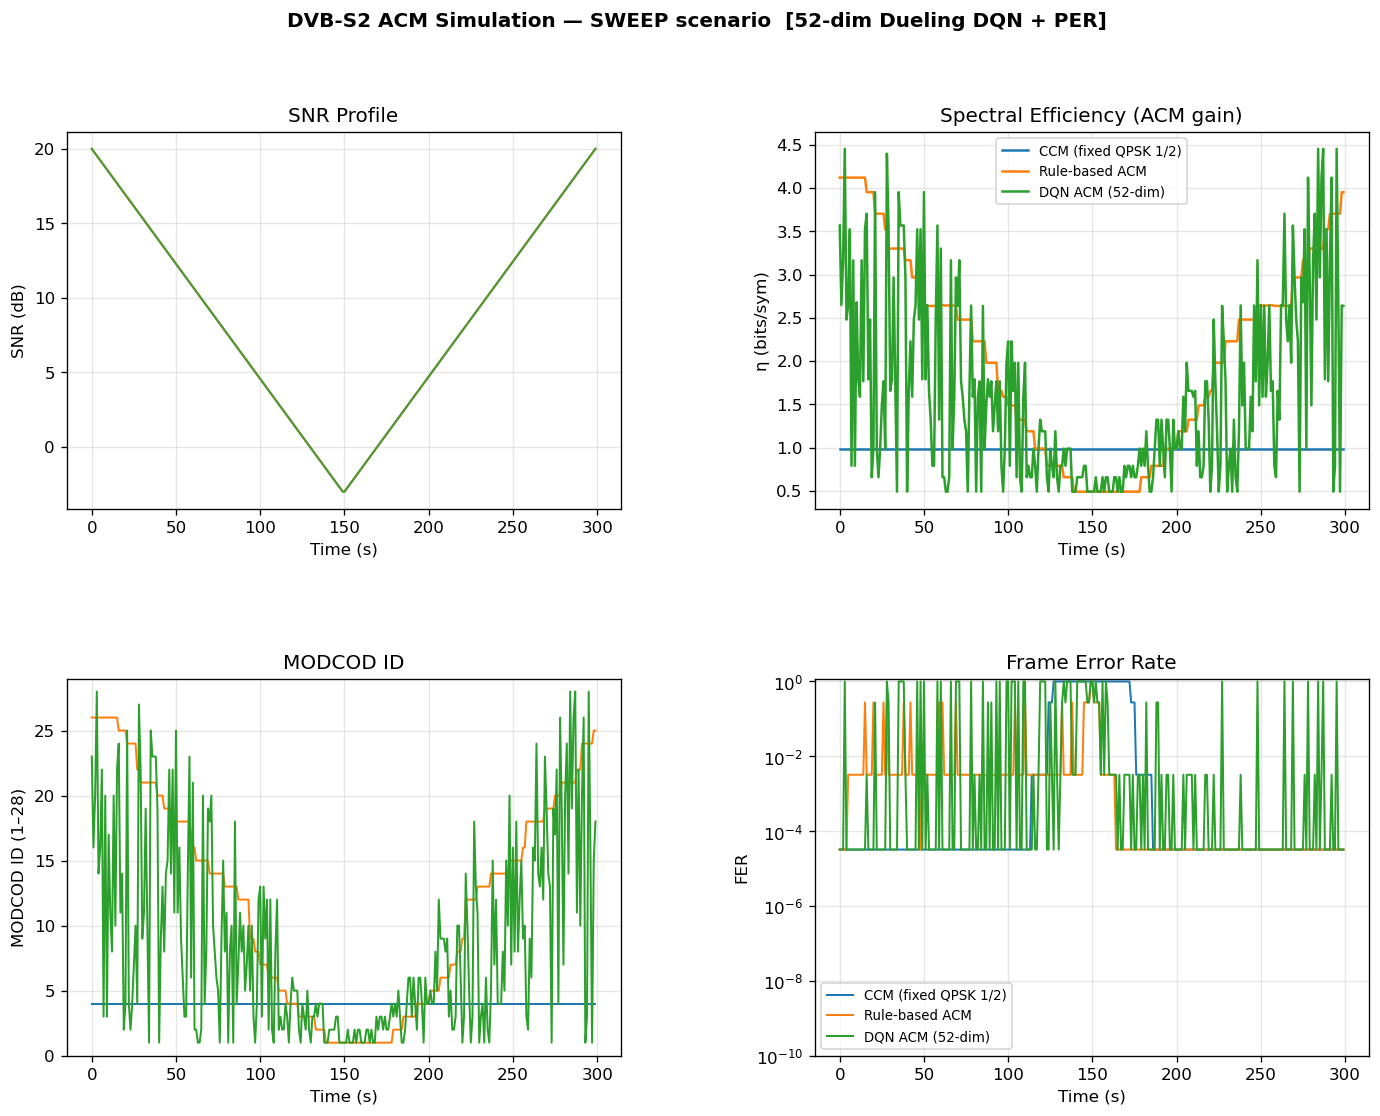
\includegraphics[width=\textwidth]{acm_simulation_results_sweep.png}
  \end{column}
  \begin{column}{0.35\textwidth}
    \vspace{0.5em}
    \textbf{Setup:} SNR linearly swept from $-3$ to $+20$\,dB and back.
    Exercises all 28 MODCODs.

    \vspace{0.8em}
    \begin{tabular}{lcc}
      \toprule
      Strategy & $\eta$ & QEF\% \\
      \midrule
      CCM        & 0.99 & 76.0 \\
      Rule-based & 2.07 & 47.3 \\
      DQN$^*$    & \textbf{1.30} & \textbf{69.3} \\
      \bottomrule
    \end{tabular}
    \vspace{0.3em}\\
    \scriptsize $^*$DQN — online training during run ($\varepsilon: 1.0 \to 0.56$)

    \vspace{0.8em}
    \begin{resultbox}{Observation}
      \small DQN trades some $\eta$ vs rule-based for significantly better link reliability (+22 pp QEF). Still early training — improving with more passes.
    \end{resultbox}
  \end{column}
\end{columns}
\end{frame}

% ── Scenario 2: LEO Pass ─────────────────────────────────────
\begin{frame}[shrink=5]{Scenario 2: LEO Pass — 9.2-Minute Orbital Arc}
\begin{columns}[T]
  \begin{column}{0.62\textwidth}
    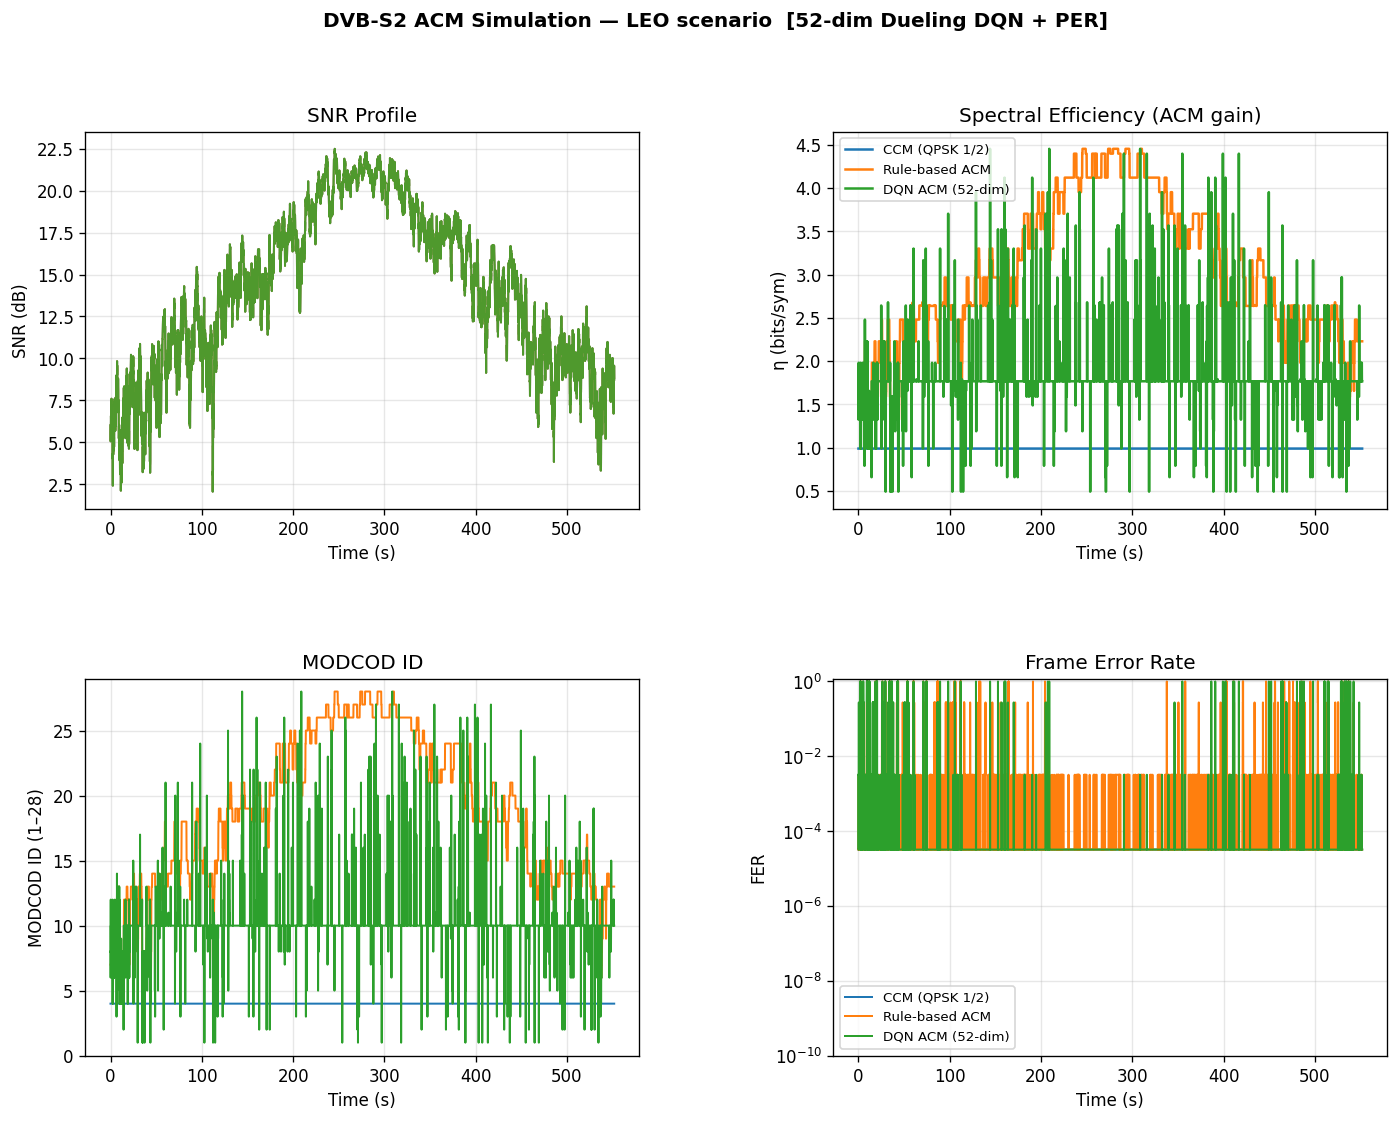
\includegraphics[width=\textwidth]{acm_simulation_results_leo.png}
  \end{column}
  \begin{column}{0.35\textwidth}
    \vspace{0.5em}
    \textbf{Setup:} Full LEO pass at 500\,km. ITU-R P.618-13 channel.
    12.2\,dB SNR swing from AOS to TCA to LOS.

    \vspace{0.8em}
    \begin{tabular}{lcc}
      \toprule
      Strategy & $\eta$ & QEF\% \\
      \midrule
      CCM        & 0.99 & 99.8 \\
      Rule-based & \textbf{3.02} & 64.2 \\
      DQN$^*$    & 1.74 & \textbf{83.3} \\
      \bottomrule
    \end{tabular}
    \vspace{0.3em}\\
    \scriptsize $^*$DQN — online training during run ($\varepsilon: 1.0 \to 0.56$)

    \vspace{0.8em}
    \begin{resultbox}{Observation}
      \small Rule-based achieves highest $\eta$ but sacrifices 35\% of frames. DQN maintains 83\% QEF while delivering $1.74\times$ CCM throughput.
    \end{resultbox}
  \end{column}
\end{columns}
\end{frame}

% ── Scenario 3: Rain Fade ────────────────────────────────────
\begin{frame}[shrink=5]{Scenario 3: Rain Fade — Graceful Degradation}
\begin{columns}[T]
  \begin{column}{0.62\textwidth}
    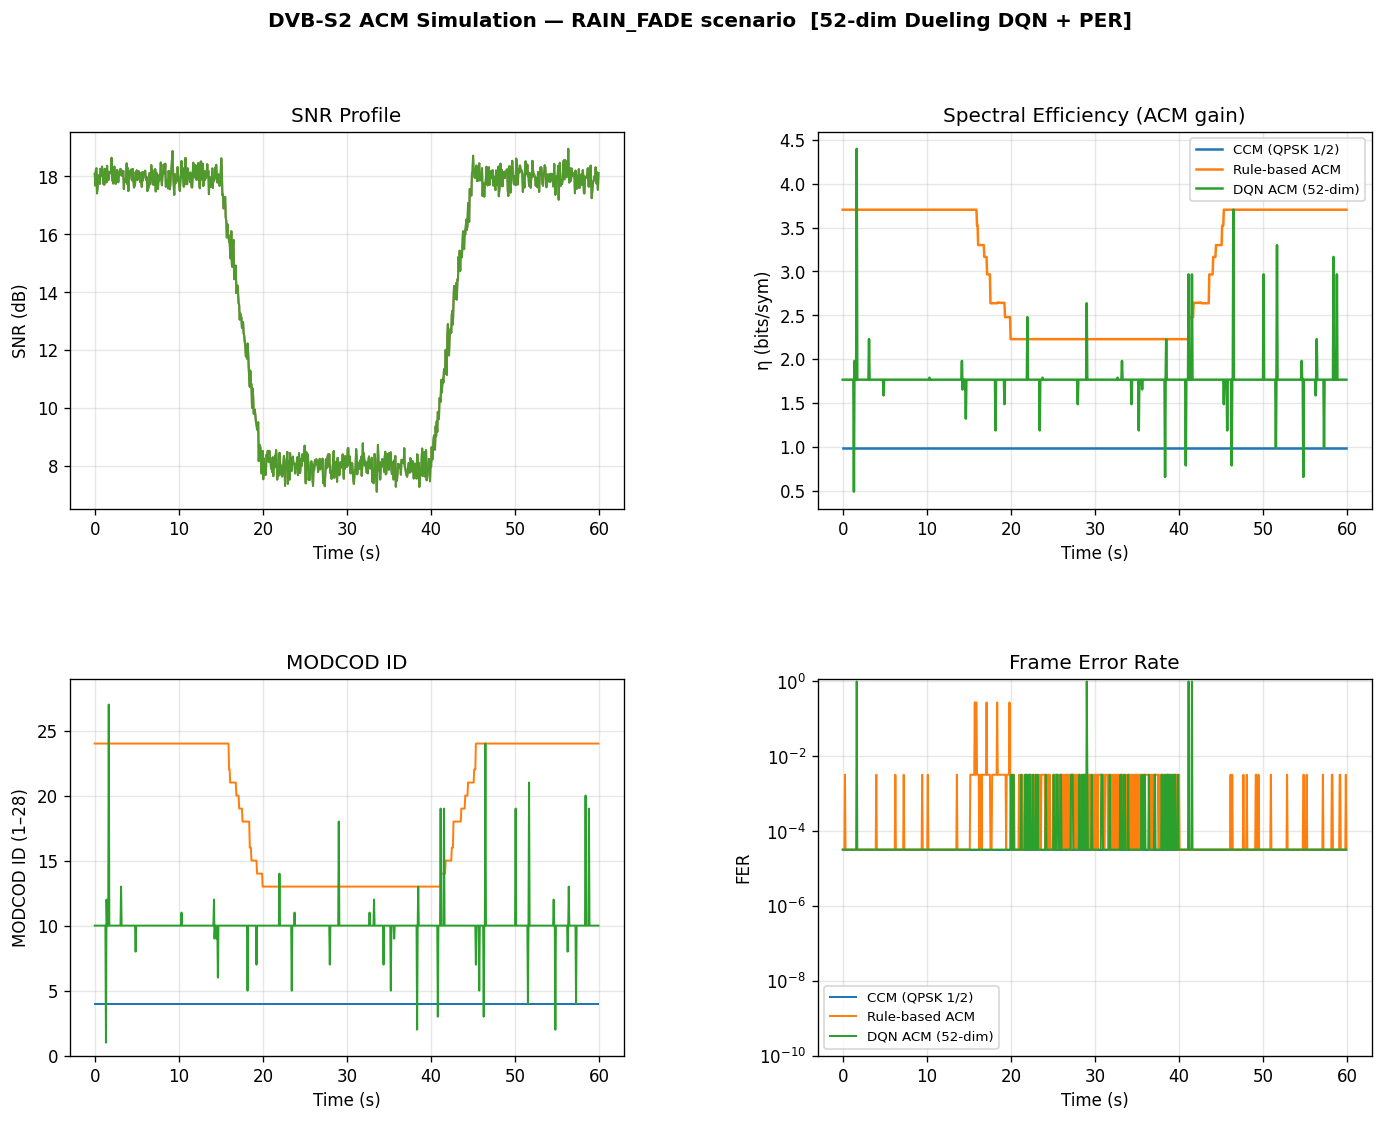
\includegraphics[width=\textwidth]{acm_simulation_results_rain_fade.png}
  \end{column}
  \begin{column}{0.35\textwidth}
    \vspace{0.5em}
    \textbf{Setup:} 10\,dB rain fade event at $t=15$\,s, recovery at
    $t=45$\,s. ITU-R P.838-3 + P.839-4 rain model.

    \vspace{0.8em}
    \begin{tabular}{lcc}
      \toprule
      Strategy & $\eta$ & QEF\% \\
      \midrule
      CCM        & 0.99 & 100.0 \\
      Rule-based & 3.07 & 68.0 \\
      DQN$^*$    & \textbf{2.01} & \textbf{88.2} \\
      \bottomrule
    \end{tabular}
    \vspace{0.3em}\\
    \scriptsize $^*$DQN — online training during run ($\varepsilon: 1.0 \to 0.56$)

    \vspace{0.8em}
    \begin{resultbox}{Observation}
      \small DQN best balances throughput and reliability under sudden fades. QEF gain of +20 pp over rule-based with $2\times$ CCM throughput.
    \end{resultbox}
  \end{column}
\end{columns}
\end{frame}

% ── Cross-Scenario Comparison ────────────────────────────────
\begin{frame}[shrink=15]{Cross-Scenario Comparison Summary \normalfont\small(DQN: online training, $\varepsilon: 1.0 \to 0.56$ across runs)}
\begin{center}
\renewcommand{\arraystretch}{1.3}
\begin{tabular}{llcccc}
  \toprule
  \textbf{Scenario} & \textbf{Strategy} & \textbf{$\eta$ (bits/sym)} &
  \textbf{Switches} & \textbf{QEF\%} \\
  \midrule
  \multirow{3}{*}{SNR Sweep}
    & CCM             & 0.99 & 0   & 76.0 \\
    & Rule-based      & 2.07 & 42  & 47.3 \\
    & \textbf{DQN}   & \textbf{1.30} & 235 & \textbf{69.3} \\
  \midrule
  \multirow{3}{*}{LEO Pass}
    & CCM             & 0.99 & 0   & 99.8 \\
    & Rule-based      & \textbf{3.02} & 393 & 64.2 \\
    & \textbf{DQN}   & 1.74 & 7076 & \textbf{83.3} \\
  \midrule
  \multirow{3}{*}{Rain Fade}
    & CCM             & 0.99 & 0  & 100.0 \\
    & Rule-based      & 3.07 & 18 & 68.0 \\
    & \textbf{DQN}   & \textbf{2.01} & 697 & \textbf{88.2} \\
  \bottomrule
\end{tabular}
\end{center}

\vspace{0.5em}
\begin{columns}[T]
  \begin{column}{0.48\textwidth}
    \begin{resultbox}{DQN strengths}
      \small
      \begin{itemize}
        \item Best QEF\% in 2 of 3 scenarios
        \item Learns to be conservative during fades
        \item Reward penalises FER heavily ($-3.0 \times \text{FER}$)
      \end{itemize}
    \end{resultbox}
  \end{column}
  \begin{column}{0.48\textwidth}
    \begin{notebox}{DQN — current limitation}
      \small
      \begin{itemize}
        \item High switch count in LEO (7076) — still exploring ($\varepsilon$-greedy)
        \item Needs more training passes to converge
        \item Online learning: improves each pass
      \end{itemize}
    \end{notebox}
  \end{column}
\end{columns}
\end{frame}

% ── TEF Summary ──────────────────────────────────────────────
\begin{frame}{Throughput Efficiency Factor (TEF)}
\begin{columns}[T]
  \begin{column}{0.55\textwidth}
    \vspace{0.3em}
    TEF captures both throughput and reliability in a single metric:
    \[
      \text{TEF} = \eta \times (1 - \text{FER}) \quad \text{[bits/sym, effective]}
    \]
    A high-$\eta$ link with many frame errors has \textit{low} effective TEF.

    \vspace{0.8em}
    \renewcommand{\arraystretch}{1.3}
    \begin{tabular}{lccc}
      \toprule
      \textbf{Strategy} & \textbf{Sweep} & \textbf{LEO} & \textbf{Rain Fade} \\
      \midrule
      CCM        & 0.75 & 0.99 & 0.99 \\
      Rule-based & 1.09 & 1.94 & 2.09 \\
      \textbf{DQN} & \textbf{0.90} & \textbf{1.45} & \textbf{1.78} \\
      \bottomrule
    \end{tabular}
  \end{column}
  \begin{column}{0.42\textwidth}
    \begin{resultbox}{Key takeaway}
      \small DQN consistently outperforms CCM in effective throughput across all scenarios. Rain fade is DQN's strongest scenario — it learns the fade pattern and pre-emptively downgrades MODCOD before outage.
    \end{resultbox}

    \vspace{0.8em}
    \begin{keybox}{Why DQN $<$ Rule in TEF}
      \small DQN is still in early training ($\varepsilon \approx 0.8$, mostly random exploration). TEF gap will close as the agent accumulates experience and $\varepsilon$ decays toward 0.05.
    \end{keybox}
  \end{column}
\end{columns}
\end{frame}
% ── GNU Radio Demo Placeholder ───────────────────────────────
\begin{frame}[shrink=10]{GNU Radio Software Loopback Demo}
\begin{columns}[T]
  \begin{column}{0.55\textwidth}
    \begin{center}
      % Inline video — plays in Adobe Acrobat Reader
      \movie[width=0.98\linewidth, height=0.55\linewidth,
             poster, showcontrols, borderwidth=1pt]{%
        
\begin{tikzpicture}
          \node[rectangle, draw=NUSblue, fill=NUSblue!8, rounded corners=4pt,
                minimum width=7.4cm, minimum height=4.15cm] {};
          \node[font=\normalsize\bfseries, NUSblue] at (0,0.5) {GNU Radio ACM Demo};
          \node[font=\small, NUSgray] at (0,0) {Click to play (Adobe Acrobat Reader)};
          \node[font=\tiny, NUSgray] at (0,-0.5) {\texttt{grc\_screen\_record.mp4}};
        \end{tikzpicture}%
      }{grc_screen_record.mp4}\\[0.3em]
      % Backup — OneDrive link for other PDF viewers
      \scriptsize\textcolor{NUSgray}{No Acrobat? $\to$\enskip}%
      \href{https://nusu-my.sharepoint.com/:f:/g/personal/manujayaugp_u_nus_edu/IgBL8WLq6Kg3T72oFts44raeAY2qRBnLZsHWS2kot5pOpYc}{%
        \textcolor{NUSorange}{$\blacktriangleright$ Watch on NUS OneDrive}}
    \end{center}
  \end{column}
  \begin{column}{0.42\textwidth}
    \vspace{0.5em}
    \textbf{Current setup:} Random source $\to$ full signal chain $\to$ AWGN channel (no USRP yet)

    \vspace{0.4em}
    \textbf{What the video shows:}
    \begin{enumerate}\small
      \item GRC flowgraph — TX chain, AWGN channel, RX chain, ACM controller
      \item Execution starts — QPSK constellation appears
      \item AWGN noise increases — MODCOD steps down\\(32APSK $\to$ 16APSK $\to$ 8PSK $\to$ QPSK)
      \item Noise reduces — link climbs back to high-order MODCOD
    \end{enumerate}

    \vspace{0.4em}
    \begin{keybox}{Key point}
      \small Full BCH+LDPC FEC, real Pilot-MMSE SNR estimation, and PLSCODE signalling — all working in software. Constellation changes \textit{automatically} with no manual intervention.
    \end{keybox}
  \end{column}
\end{columns}
\end{frame}

% ── Constellation Screenshots Placeholder ────────────────────
\begin{frame}[shrink=5]{GNU Radio: Constellation at Each MODCOD}
\begin{center}
\small\textit{Screenshots from GNU Radio Qt GUI — to be inserted from screen recording}
\end{center}
\vspace{0.3em}
\begin{columns}[T]
  \begin{column}{0.23\textwidth}
    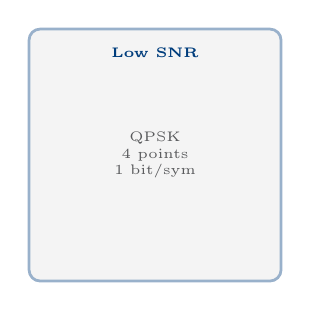
\begin{tikzpicture}
      \draw[NUSblue!40, fill=NUSlightgray, rounded corners=4pt, line width=1pt]
        (0,0) rectangle (3.2,3.2);
      \node[font=\tiny, NUSgray, align=center] at (1.6,1.6)
        {QPSK\\4 points\\1 bit/sym};
      \node[font=\tiny\bfseries, NUSblue] at (1.6,2.9) {Low SNR};
    \end{tikzpicture}
  \end{column}
  \begin{column}{0.23\textwidth}
    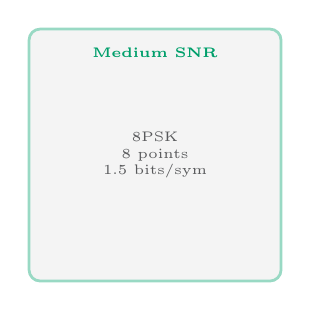
\begin{tikzpicture}
      \draw[NUSgreen!40, fill=NUSlightgray, rounded corners=4pt, line width=1pt]
        (0,0) rectangle (3.2,3.2);
      \node[font=\tiny, NUSgray, align=center] at (1.6,1.6)
        {8PSK\\8 points\\1.5 bits/sym};
      \node[font=\tiny\bfseries, NUSgreen] at (1.6,2.9) {Medium SNR};
    \end{tikzpicture}
  \end{column}
  \begin{column}{0.23\textwidth}
    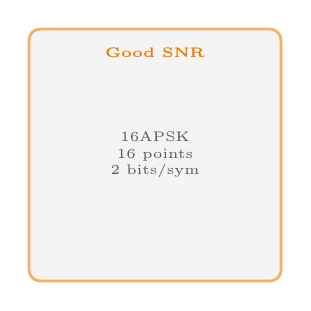
\begin{tikzpicture}
      \draw[NUSorange!60, fill=NUSlightgray, rounded corners=4pt, line width=1pt]
        (0,0) rectangle (3.2,3.2);
      \node[font=\tiny, NUSgray, align=center] at (1.6,1.6)
        {16APSK\\16 points\\2 bits/sym};
      \node[font=\tiny\bfseries, NUSorange] at (1.6,2.9) {Good SNR};
    \end{tikzpicture}
  \end{column}
  \begin{column}{0.23\textwidth}
    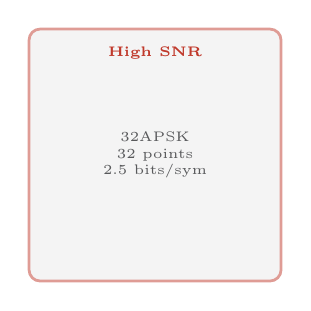
\begin{tikzpicture}
      \draw[NUSred!50, fill=NUSlightgray, rounded corners=4pt, line width=1pt]
        (0,0) rectangle (3.2,3.2);
      \node[font=\tiny, NUSgray, align=center] at (1.6,1.6)
        {32APSK\\32 points\\2.5 bits/sym};
      \node[font=\tiny\bfseries, NUSred] at (1.6,2.9) {High SNR};
    \end{tikzpicture}
  \end{column}
\end{columns}

\vspace{0.8em}
\begin{columns}[T]
  \begin{column}{0.55\textwidth}
    \begin{notebox}{How to read the constellation}
      \small Each dot is a received IQ symbol. Tight clusters = high SNR, good link.
      Spread/overlapping clusters = low SNR or wrong MODCOD selected.
      The ACM system keeps clusters tight by choosing the right MODCOD.
    \end{notebox}
  \end{column}
  \begin{column}{0.42\textwidth}
    \begin{resultbox}{What to look for in the video}
      \small As SNR drops: constellation transitions from 32APSK (dense) $\to$ QPSK (4 clear points). The link stays connected throughout.
    \end{resultbox}
  \end{column}
\end{columns}
\end{frame}
% ── Conclusions ───────────────────────────────────────────────
\begin{frame}{Summary}
\begin{columns}[T]
  \begin{column}{0.55\textwidth}
    \begin{enumerate}\small
      \item[\textbf{1.}] \textbf{CCM is safe but wasteful} — QEF near 100\% but
        $\eta = 0.99$ bits/sym always. Leaves most link capacity unused.
      \vspace{0.4em}
      \item[\textbf{2.}] \textbf{Rule-based ACM maximises $\eta$} but sacrifices
        reliability — up to 35\% frame loss in LEO scenario.
      \vspace{0.4em}
      \item[\textbf{3.}] \textbf{DQN ACM balances both} — best QEF\% in 2/3
        scenarios, $2\times$ CCM throughput in rain fade. Still converging
        (more training $\to$ better $\eta$).
      \vspace{0.4em}
      \item[\textbf{4.}] \textbf{GNU Radio software loopback confirms} the full signal chain works — real LDPC, real SNR estimation, constellation changes automatically. USRP B200 hardware connection is the next step.
    \end{enumerate}
  \end{column}
  \begin{column}{0.42\textwidth}
    \begin{resultbox}{Best result}
      \small Rain fade scenario: DQN achieves\\
      $\eta = 2.01$ bits/sym with QEF $= 88.2\%$\\
      vs rule-based QEF $= 68.0\%$\\[0.3em]
      \textbf{+20 percentage points} reliability\\with $2\times$ CCM throughput.
    \end{resultbox}

    \vspace{0.5em}
    \begin{keybox}{Next step}
      \small Connect USRP B200 hardware and run \texttt{acm\_loopback.grc} over a real X-Band link for IoV validation (March 2026).
    \end{keybox}
  \end{column}
\end{columns}
\end{frame}

\end{document}
